\newdimen\nodeDist
\nodeDist=35mm

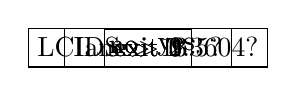
\begin{tikzpicture}[
    node/.style={%
      draw,
      rectangle,
    },
  ]

    \node [node] (A) {IDS $>$ 13.5?};
    \path (A) ++(-135:\nodeDist) node [node] (B) {exit 1};
    \path (A) ++(-45:\nodeDist) node [node] (C) {LCIanx $>$ 0.3604?};
    \path (C) ++(-135:\nodeDist) node [node] (D) {exit 2};
    \path (C) ++(-45:\nodeDist) node [node] (E) {exit 3};

    \draw (A) -- (B) node [left,pos=0.25] {no}(A);
    \draw (A) -- (C) node [right,pos=0.25] {yes}(A);
    \draw (C) -- (D) node [left,pos=0.25] {no}(A);
    \draw (C) -- (E) node [right,pos=0.25] {yes}(A);
\end{tikzpicture}